
From the given information, 
% \begin{align}
% \myvec{3 & -1 & 2}\vec{x}&=4 \label{linform/39/2.0.1}
% \\
% \myvec{1 & 1 & 1}\vec{x}&=-2 \label{linform/39/2.0.2}
% \\
% \vec{A}&=\myvec{2 \\ 2 \\ 1} \label{linform/39/2.0.3}
% \end{align}
% %
% Equation can be written as,
% \begin{align}
% \vec{n_1^T}\vec{x} &= c_1 \label{linform/39/2.0.4}\\
% \vec{n_2^T}\vec{x} &= c_2 \label{linform/39/2.0.5}
% \end{align}
% Where,
\begin{align}
\vec{n_1}&=\myvec{3 \\ -1 \\ 2},\vec{n_2}=\myvec{1 \\ 1 \\ 1}
\\
c_1&=4,c_2=-2
\end{align}
The intersection of the planes is given by 
%Required equation of the plane containing \eqref{linform/39/2.0.4} and \eqref{linform/39/2.0.5} is,
\begin{align}
\vec{n_1^T}\vec{x} + \lambda\vec{n_2^T}\vec{x}  &= c_1+\lambda c_2  \\ 
\implies (\vec{n_1^T}+\lambda\vec{n_2^T})\vec{x} &= c_1+\lambda c_2 \label{linform/39/2.0.9}
\end{align}
yielding 
%By substituting the intersection of the plane of the point \eqref{linform/39/2.0.3}.so,
\begin{align}
\lambda&=\frac{(c_1-\vec{A}\vec{n_1^T})}{(\vec{A}\vec{n_2^T}-c_2)} \\
%&=\frac{4-\myvec{2\\2\\1}\myvec{3 & -1 & 2}}{\myvec{2\\2\\1}\myvec{1 & 1 & 1}+2}\\
 &= \frac{-2}{7}
\end{align}
$\therefore $ By substituting the numerical values in  \eqref{linform/39/2.0.9}, the desired  equation of the plane is 
\begin{align}
\myvec{19 & -9 & 12}\vec{x} = 32 
\end{align}
which is plotted in Fig. \ref{linform/39/Plot of the plane}
%
\begin{figure}[!ht]
\centering
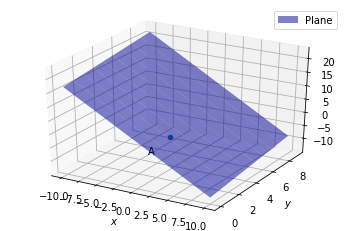
\includegraphics[width=\columnwidth]{solutions/su2021/2/39/Plane_plot.png}
\caption{Plot of the plane}
\label{linform/39/Plot of the plane}
\end{figure}

